\chapter{Redes de interacción entre tortugas}
\graphicspath{{figs/}}
 
\chapterquote{There are times in any science that a transformation to deeper understanding is pressing upward in some as yet poorly articulated form. We may be in such a period in biology.}{Stuart A. Kauffman, 1993}
 
\label{Redes de interacción entre tortugas}
\section{Trayectorias }
 
En la Fig.~\ref{fig:trayeSinFiltr} se muestran las trayectorias obtenidas de los datos crudos en el día de medición 1/12/2020. Para graficar el mapa de las trayectorias se realizó un programa en el lenguaje Python utilizando la librería Folium \cite{github}.
 
\begin{figure}[ht]
    \begin{center}
       
   
    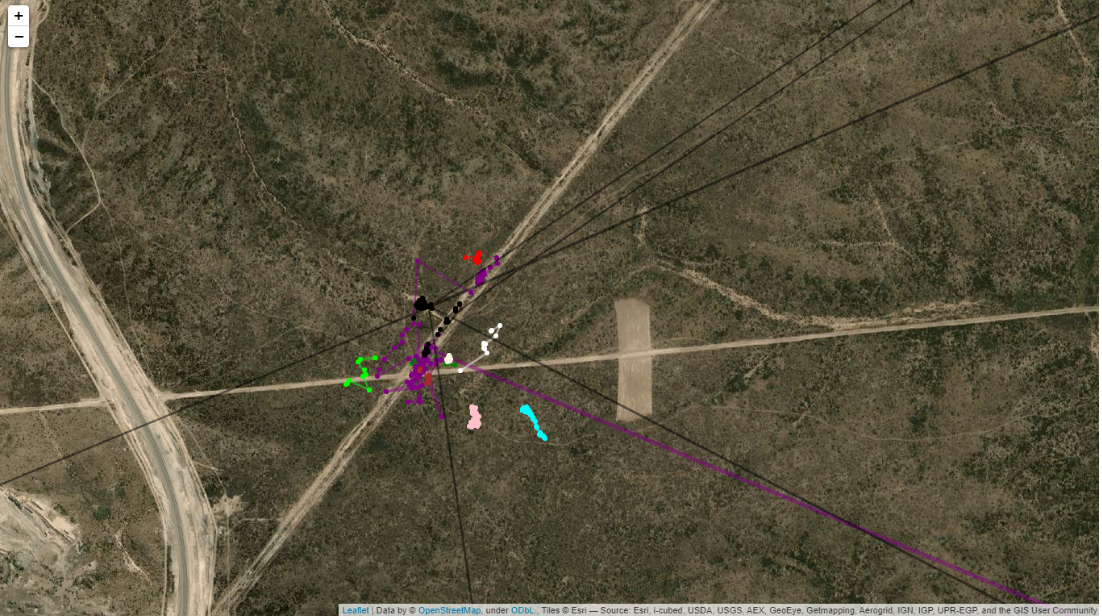
\includegraphics[width=\imsize]{Chap2/Traye1_12_sinF.png}
\end{center}
    \caption[Trayectorias un dia de medición, sin filtrar.]{Trayectorias del 1/12/2020; cada color representa una tortuga diferente. Ambas metodologías fueron implementadas; algunos puntos tomados con el tortugómetro escapan a la trayectoria esperada.}
    \label{fig:trayeSinFiltr}
\end{figure}
Se observa en la Fig.~\ref{fig:trayeSinFiltr}, que algunos puntos tomados por el tortugómetro se desvían de la trayectoria esperada para una tortuga (recorren distancias del orden de los kilómetros en menos de 10 minutos). Se estima que estas desviaciones se producen por dos motivos: en primer lugar, en los primeros minutos de medición, el GPS comienza a conectarse a satélites hasta tener la precisión máxima, haciendo que  los primeros puntos tengan una mayor desviación; en segundo lugar, se observó de manera aleatoria la desviación de algún punto respecto de la trayectoria típica. Para filtrar estas desviaciones, se implementó un método basado en la velocidad máxima que pueden alcanzar los individuos. El mismo está detallado en el repositorio de GitHub, archivo \textit{CriterioParaSacarData.py} \cite{github}. Para obtener la velocidad máxima se calculó la distribución de velocidades de la Fig.~\ref{fig:distribuciondeVel}.
 
 
\begin{figure}[ht]
\begin{center}
       
   
    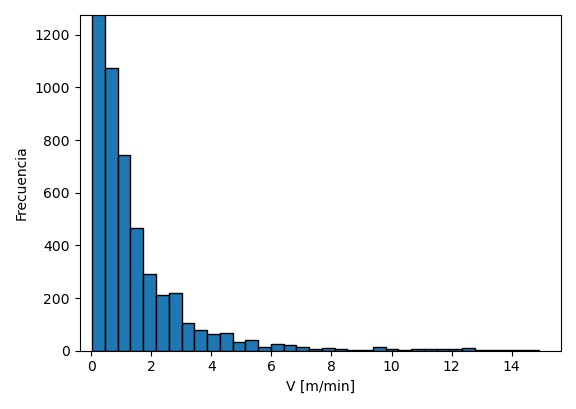
\includegraphics[width=1.2\imsize]{Chap2/Velocidades3.jpeg}
    \caption[Distribución de velocidades.]{Histograma de velocidades en m/min. Las  velocidades obtenidas mayores a 15 m/min están órdenes de magnitud por encima y fueron descartadas.}%re hacer figuras
    \label{fig:distribuciondeVel}
\end{center}
\end{figure}
Se observó en la distribución de velocidades de la Fig.~\ref{fig:distribuciondeVel}, que las tortugas llegan a una velocidad máxima de aproximadamente 15m/min, de manera que se adoptó el criterio de filtrar los tramos de trayectoria en los que la velocidad supera ese valor máximo. Filtrando los puntos de la Fig.~\ref{fig:trayeSinFiltr}, tomando velocidad máxima 15 m/min, se obtuvo  el mapa de la Fig.~\ref{fig:trayeConFiltr}.
 
 
 
 
\begin{figure}[ht]
    \begin{center}
       
   
    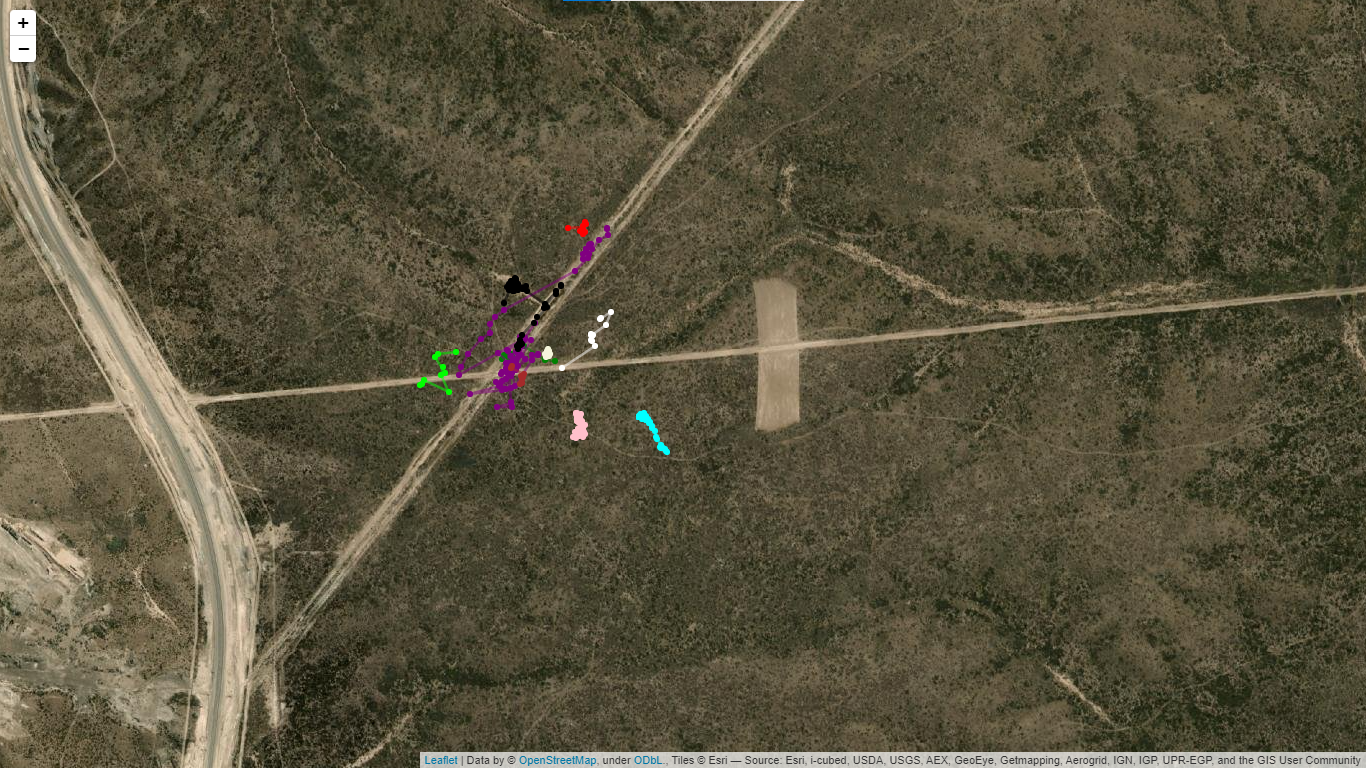
\includegraphics[width=\imsize]{Chap2/Traye1_12_conF.png}
\end{center}
    \caption[Trayectorias un dia de medición, después del filtrado.]{Trayectorias del 1/12/2020 luego del filtrado; cada color representa una tortuga diferente.}
    \label{fig:trayeConFiltr}
\end{figure}
 
\section{Zonas de interés}
Partiendo de las trayectorias filtradas, se realizó  una grilla identificando las zonas de recurrencia en la Fig.~\ref{fig:grilla1}. Las celdas de la grilla fueron elegidas de 10\,m$^2$ debido a que se estima en 10\,m el erorr del GPS del tortugómetro y se está revisando para ambas modalidades el valor del mismo. Para cada celda se contó el numero de veces que estuvo allí, la grilla fue programada en Python \cite{github}. En caso de que se pudieran identificar los factores o características de las zonas más recurridas, se podrían sugerir políticas de manejo para minimizar los daños sobre las tortugas. Esto es especialmente importante dado que ahora se está introduciendo ganado en la zona con el consiguiente deterioro del hábitat natural de las mismas.
 
 
\begin{figure}[ht]
    \begin{center}
    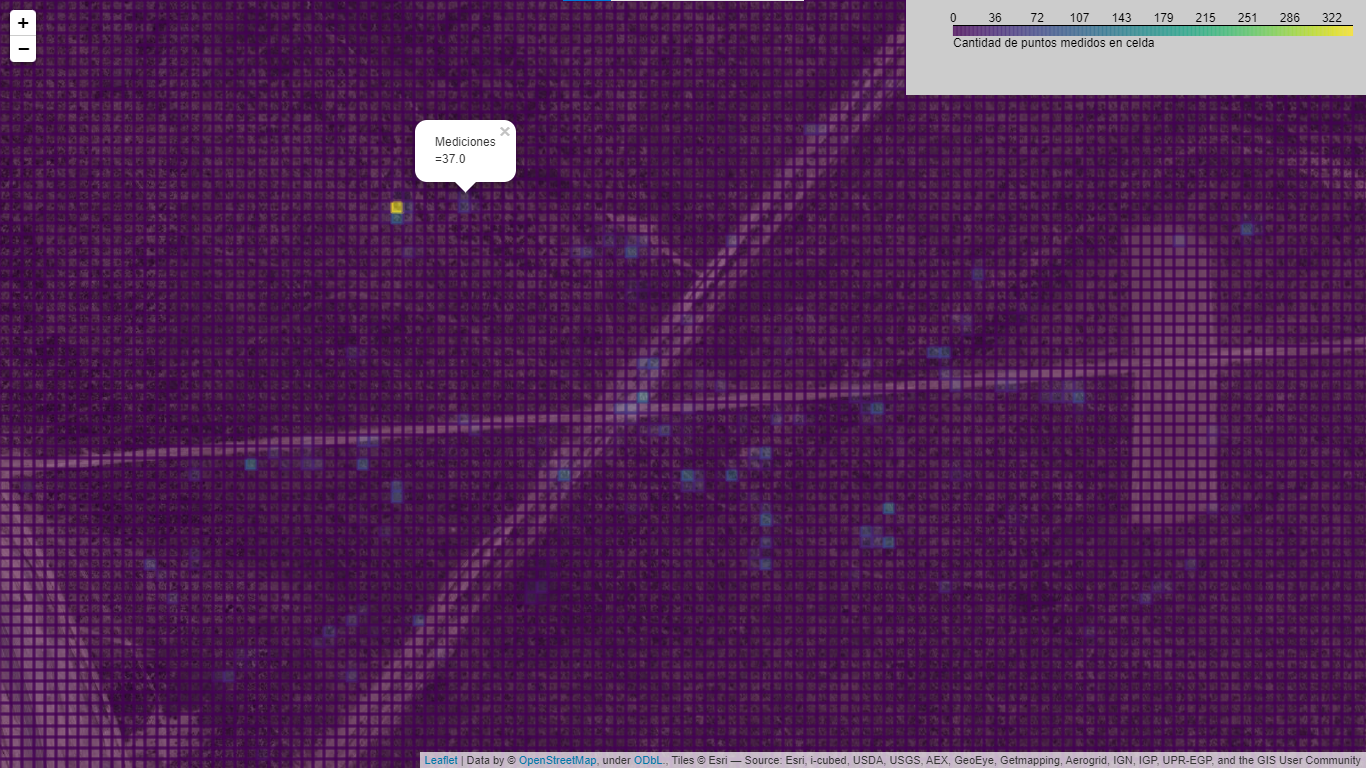
\includegraphics[width=\imsize]{Chap2/GrillaSintCNoche.png}
    \end{center}
    \caption[Mapa de zonas de recurrencia.]{Mapa de recurrencias  interactivo con las trayectorias filtradas. Al hacer clic en cualquier celda de la grilla un cartel dice cuantas mediciones fueron tomadas. El tamaño de celda es de 10m$^2$.}
    \label{fig:grilla1}
\end{figure}
 
Se puede observar en la Fig.~\ref{fig:grilla1} un punto que se destaca mucho más que el resto (arriba a la izquierda) teniendo el máximo de mediciones en esa casilla. Esto se debe a que una pareja de tortugas pasó la noche con el tortugómetro puesto en medio de un arbusto de difícil acceso. Para obtener una mejor idea de las zonas de interés diurnas se realizó otra grilla usando sólo datos del tortugómetro registrados en el día (entre 7am y 9pm) y  realizando una interpolación lineal de 1 punto por minuto por cada par de puntos consecutivos (Fig.~\ref{fig:grillaInt}, \cite{github}). Esta interpolación da una aproximación de las casillas por donde tuvo que pasar la tortuga y añade un peso cuando la tortuga se quedó dentro de la misma casilla por una mayor cantidad de tiempo (mediciones consecutivas).
 
\begin{figure}[ht]
    \begin{center}
       
   
    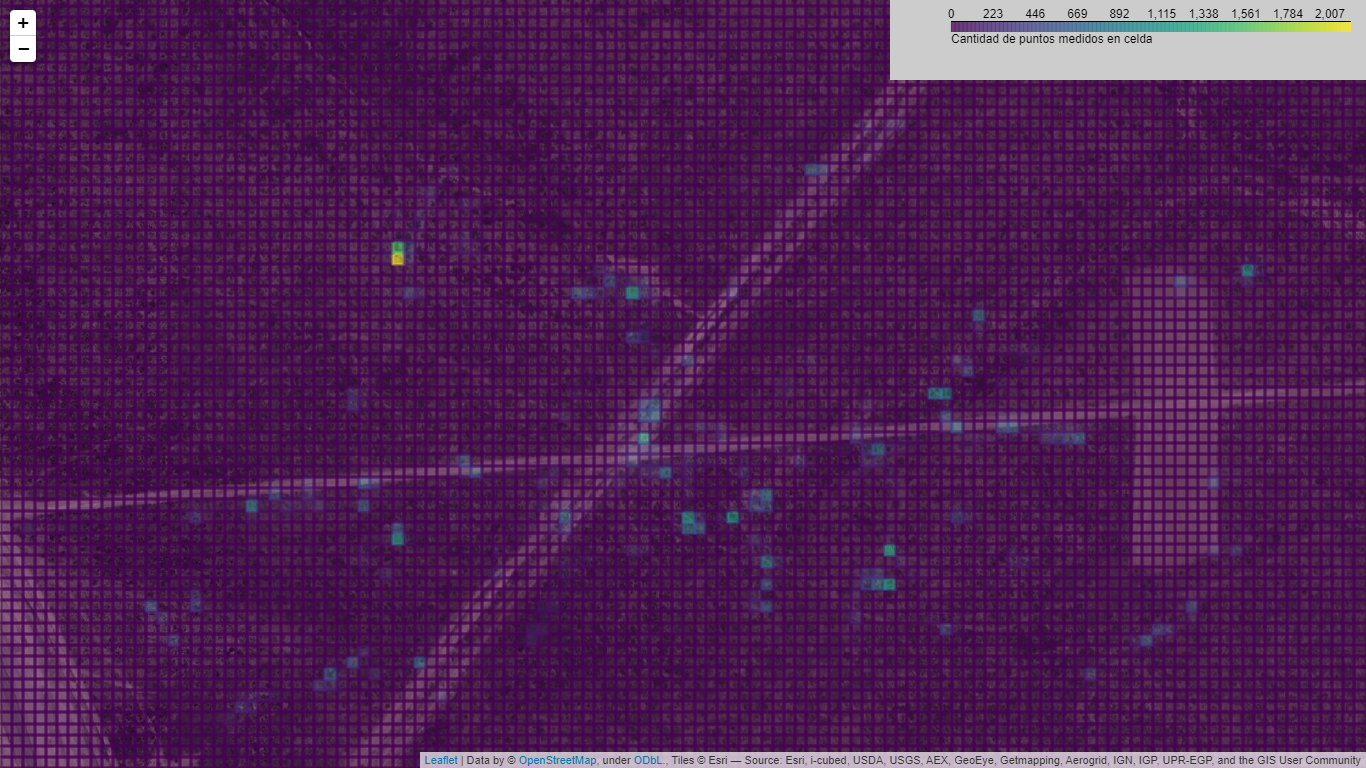
\includegraphics[width=\imsize]{Chap2/GrillaCintSNoche.png}
\end{center}
    \caption[Mapa con zona de recurrencia para trayectorias diurnas.]{Mapa de recurrencias  interactivo con las trayectorias diurnas (7am-9pm) filtradas e interpoladas linealmente. Al hacer clic en cualquier celda de la grilla un cartel dice cuantas mediciones fueron tomadas. El tamaño de celda es de 10m$^2$.}
    \label{fig:grillaInt}
\end{figure}


Comparando las Figs. \ref{fig:grilla1} y \ref{fig:grilla1}, se observa en la  Fig.~\ref{fig:grillaInt} un mayor contraste de las otras celdas respecto al que se encuentra arriba a la izquierda. Esto se debe a la extracción de los puntos nocturnos. Al momento se desconocen los motivos por los cuales dichas zonas son muy visitadas, esto será investigado en profundidad en el futuro.
 
\section{Red de encuentros}
Partiendo de las trayectorias filtradas, se decidió buscar el solapamiento de las trayectorias, para identificar los encuentros. Para ello, se implementó un código en Python que, partiendo de cualquier punto de su trayectoria, busca si hay otro punto de otra tortuga que se encuentre a una distancia menor a 20 metros (se estima que el error del GPS es de 10\,m) y a una distancia temporal menor a 20 minutos. Cuando se cumple esta condición se van guardando los pares de puntos junto con la hora y el nombre de ambas tortugas.
 
En las Figs. \ref{fig:encuentros_hora_medida_tortugometro} y \ref{fig:encuentros_hora_medida_igotu}, pueden verse la cantidad de encuentros calculados por hora medida por los tortugómetros y por los i-gotU en función de los meses de medición. Los encuentros del tipo macho-hembra fueron normalizados por la cantidad promedio de horas medidas de ambos sexos para cada mes, en cambio para la cantidad de encuentros macho-macho y hembra-hembra se normalizó utilizando la cantidad de horas medidas para cada sexo en cada mes.  
\begin{figure}[ht]
    \begin{center}
       
   
    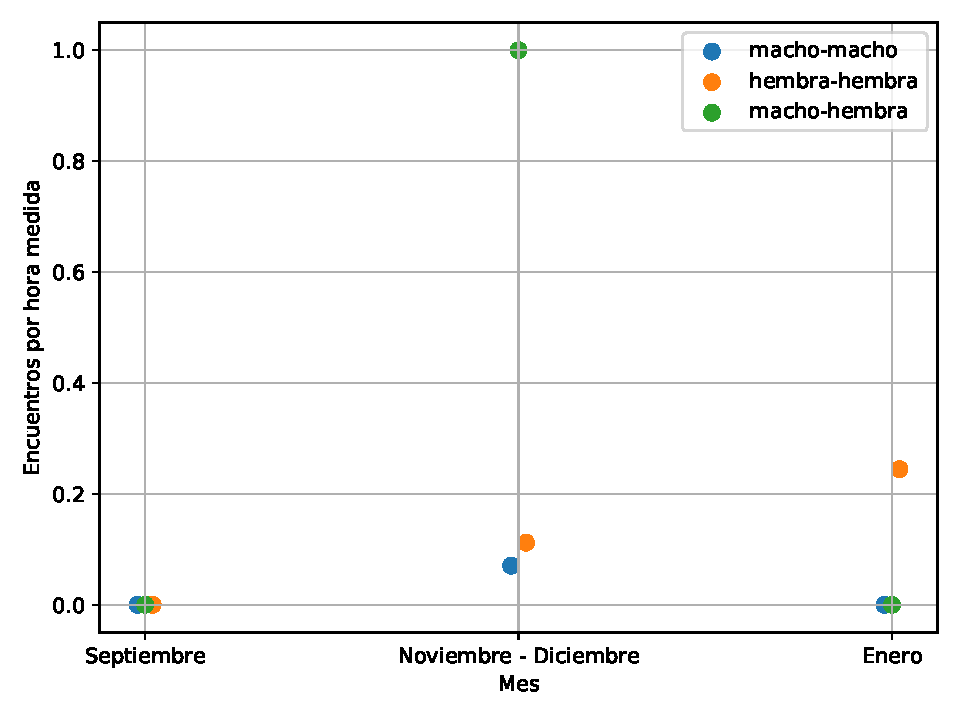
\includegraphics[width=\imsize]{Chap2/encuentros_por_hora_tortugometro.pdf}
\end{center}
    \caption[Encuentros por hora medida tomando los datos del tortugómetro.]{Encuentros sobre cantidad de horas medidas para cada sexo en función de los meses de medición utilizando el tortugómetro. Los distintos colores identifican el tipo de encuentro.}
    \label{fig:encuentros_hora_medida_tortugometro}
\end{figure}
 
\begin{figure}[ht]
    \begin{center}
       
   
    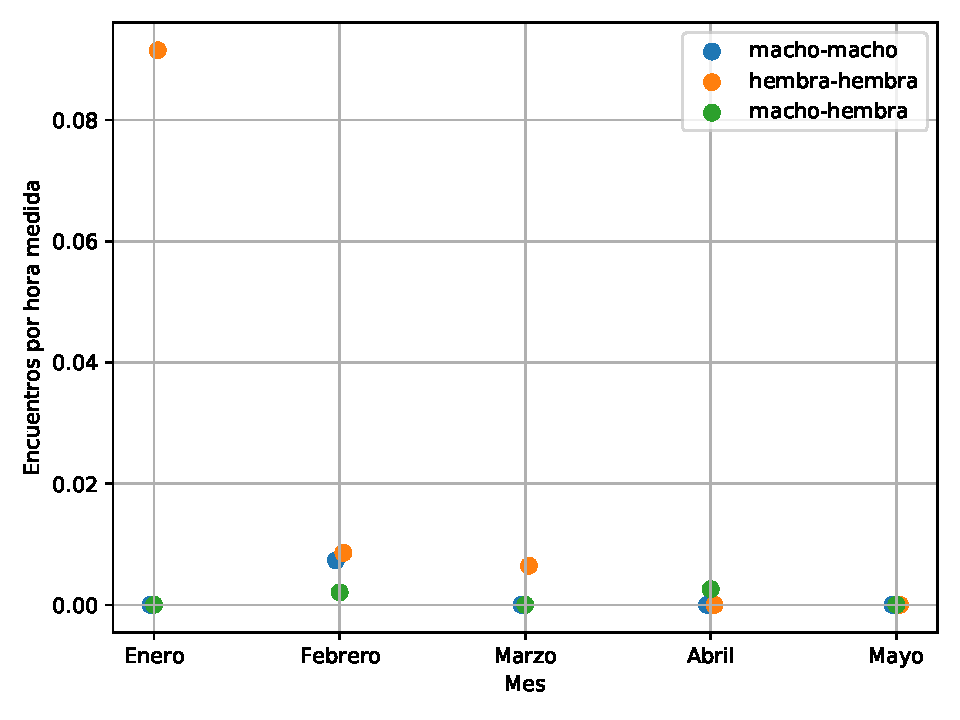
\includegraphics[width=\imsize]{Chap2/encuentros_por_hora_igotu.pdf}
\end{center}
    \caption[Encuentros por hora medida tomando los datos de los i-gotU.]{Encuentros sobre cantidad de horas medidas para cada sexo en función de los meses de medición utilizando los i-gotU. Los distintos colores identifican el tipo de encuentro.}
    \label{fig:encuentros_hora_medida_igotu}
\end{figure}
En la Fig. \ref{fig:encuentros_hora_medida_tortugometro}, se observa que el máximo de encuentros del tipo macho-hembra por hora medida ocurre en los meses noviembre-diciembre; esto coincide con la época de apareamiento. Estos meses están juntos, ya que las mediciones en esos meses fueron tomadas a finales de noviembre y principios de diciembre. Para el mes de enero solo se registraron encuentros del tipo hembra-hembra en ambas figuras ( \ref{fig:encuentros_hora_medida_tortugometro} y \ref{fig:encuentros_hora_medida_igotu}), esto puede deberse a que las hembras están buscando un lugar acorde para depositar sus huevos, haciendo el encuentro hembra-hembra más probable. Para los datos de los i-gotU (\ref{fig:encuentros_hora_medida_igotu}) también se registraron encuentros en los meses de febrero, marzo y abril, pero en menor cantidad que en los meses anteriores, asociamos esta diferencia a la disminución de actividad en las tortugas propia de este periodo.
 
 
Utilizando los encuentros calculados, se armaron dos redes de interacción  utilizando la librería NetworkX \cite{networkx}, una para los datos obtenidos con  tortugómetro y otra para los datos provenientes de i-gotU (Figs. \ref{fig:redInteraccion20mincampanas} y \ref{fig:redInteraccion20igotu}). Las conexiones entre nodos tortugas tienen peso linealmente dependiente de la cantidad de encuentros entre ellas, esto se observa en el grosor del link entre dos tortugas y las distancias relativas entre nodos.
 
 
\begin{figure}[ht]
    \begin{center}
       
   
    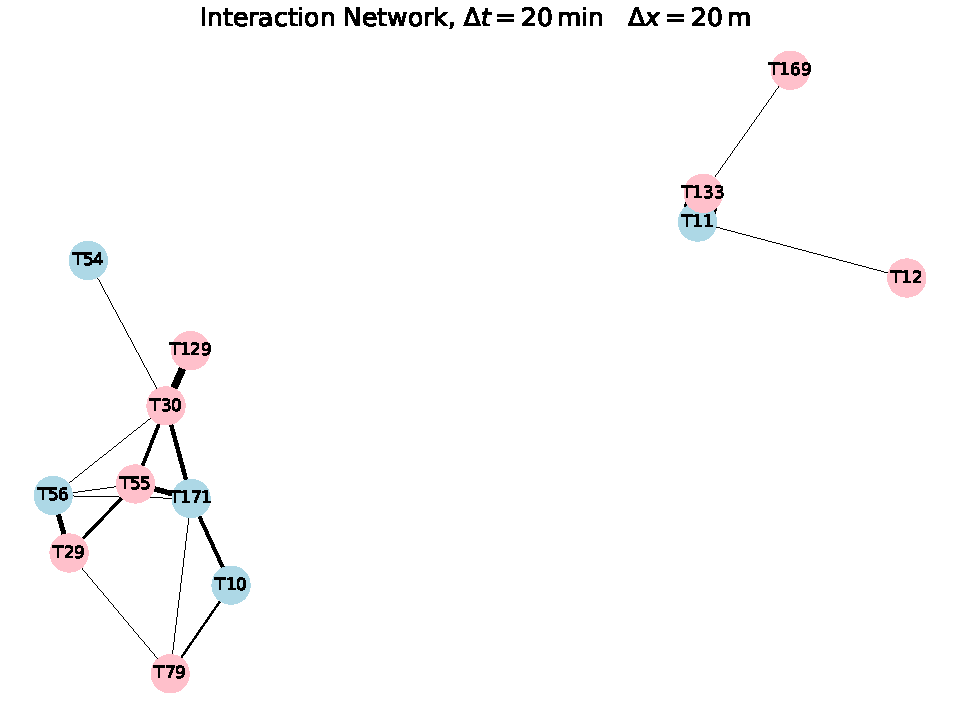
\includegraphics[width=\imsize]{Chap2/red_interaccion_20min_campanas.pdf}
\end{center}
    \caption[Red de encuentros entre tortugas  con datos tomados por el tortugómetro.]{Red de encuentros entre tortugas para datos provenientes de la metodología  tortugómetro. La condición de encuentro está dada por una distancia espacial menor a 20 metros y a una distancia temporal menor a 20 minutos. Los datos de tortugómetros fueron tomados en distintas campañas en los meses de octubre, noviembre, diciembre y mediados de enero.}
    \label{fig:redInteraccion20mincampanas}
\end{figure}
 
 
 
\begin{figure}[ht]
    \begin{center}
       
   
    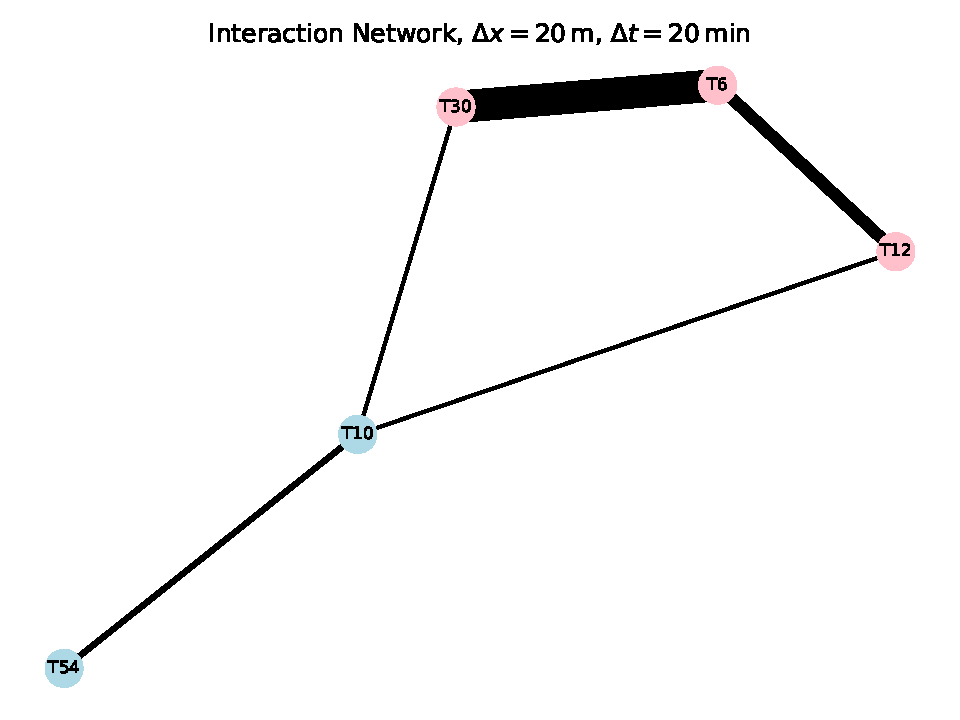
\includegraphics[width=\imsize]{Chap2/red_interaccion_20min_IGOTO.pdf}
\end{center}
    \caption[Red de encuentros entre tortugas utilizando i-gotU.]{Red de encuentros entre tortugas para datos provenientes de las metodologías i-gotU. La condición de encuentro está dada por una distancia espacial menor a 20 metros y a una distancia temporal menor a 20 minutos. Los datos de los i-gotU fueron tomados desde finales de febrero hasta principios de mayo.}
    \label{fig:redInteraccion20igotu}
\end{figure}
 
 
En la Fig. \ref{fig:redInteraccion20mincampanas}, se observa que la red de interacción está compuesta por dos comunidades. Sobre estas comunidades, se calcularon la media de las posiciones de cada nodo tortuga junto con su desviación estándar y no se encontraron diferencias significativas en estos valores para  nodos tortugas pertenecientes a cada una de las comunidades. Esto nos indica que las tortugas que pertenecen a cada comunidad, no están separadas en el espacio y no es la causa de la separación de la red en dos comunidades. Queda a determinar en futuros trabajos si la separación de la red en estas dos comunidades está relacionada con la cantidad de  mediciones o con alguna característica de la población de tortugas estudiada. En la red, también se observan diferencias  de grado, teniendo algunas tortugas muchas más conexiones que otras. Se seguirá trabajando para identificar comportamientos particulares de las tortugas que puedan estar relacionados con la distribución de grado de la red.
 
En la Fig. \ref{fig:redInteraccion20igotu}, se observa una mayor cantidad de encuentros entre las tortugas hembras (grosor de enlace), esto puede deberse a la época de medición, ya que en enero las tortugas hembras están en búsqueda de algún lugar para depositar sus huevos. En el siguiente capítulo se analizarán redes bipartitas de refugios y se compararán con las redes de interacción de tortugas para entender mejor este aspecto.
 
%%% Local Variables:
%%% mode: latex
%%% TeX-master: "template"
%%% End:
 
 
 

